\documentclass[11pt,a4paper]{article}
\usepackage[margin=2.54cm]{geometry}
\usepackage{times}
\usepackage{amsmath,amssymb}
\usepackage{graphicx}
\usepackage{booktabs}
\usepackage{multirow}
\usepackage{hyperref}
\usepackage{natbib}
\usepackage{xcolor}
\usepackage{caption}
\usepackage{setspace}
\usepackage{microtype}
\usepackage{tikz}
\usetikzlibrary{arrows.meta,positioning,fit,calc}
\usepackage{pgfplots}
\pgfplotsset{compat=1.18}
\onehalfspacing

\hypersetup{colorlinks=true,linkcolor=blue,citecolor=blue,urlcolor=blue}

\title{\textbf{Supplementary Information}\\[4pt]
\large Dissecting Sequence, Structure, and Data Recency Effects\\
in Enzyme Commission Prediction under Temporal Distribution Shift}
\author{Seunghyon Kim\\
School of Applied AI and Entrepreneurship, Handong Global University\\
Pohang, 37554, Republic of Korea\\
\texttt{jamesksh0130@gmail.com}\\
ORCID: 0009-0002-0708-748X}
\date{}

\begin{document}
\maketitle
\tableofcontents
\newpage

% ─────────────────────────────────────────────────────────────────────────────
\section*{S1\quad Related Work}
\addcontentsline{toc}{section}{S1\quad Related Work}
% ─────────────────────────────────────────────────────────────────────────────

\paragraph{Classical sequence alignment.}
Before machine learning, enzyme function annotation relied primarily on
sequence similarity transfer.
BLAST~\citep{altschul1990} identifies homologous proteins by computing pairwise
alignment scores against curated databases such as UniProtKB/Swiss-Prot;
a query enzyme is annotated with the EC number of its closest hit above an
e-value threshold.
On the EC-Bench temporal test set, BLASTp achieves a weighted F1 of 0.502 at
the 100\% similarity threshold, dropping to 0.431 when training is restricted
to proteins with at most 30\% sequence identity to the test
set~\citep{davoudi2026}---illustrating the well-known fragility of
alignment-based methods for evolutionarily distant queries.
Profile-based methods such as PRIAM mitigate this limitation through
position-specific scoring matrices derived from multiple sequence alignments,
but they cannot integrate non-sequence information such as tertiary structure.

\paragraph{Deep learning for EC prediction.}
DeepEC~\citep{ryu2019} and DEEPre introduced 1D CNNs over one-hot amino acid
sequences with global average pooling; while effective for EC Levels~1--3,
these models struggle at Level~4 due to fine-grained specificity requirements
and limited receptive fields.
ECPick~\citep{han2024} augments a hierarchical 1D CNN with Dempster--Shafer
evidential theory, assigning a trustworthiness score to each prediction.
CLEAN~\citep{yu2023} reframes EC prediction as metric learning: ESM-1b embeddings
are projected into a shared latent space trained with a triplet margin loss.
HIT-EC~\citep{dumontet2026} designs a four-level Transformer achieving micro F1 of
0.93 on Swiss-Prot---the current state of the art for sequence-only EC prediction.

\paragraph{Protein language model encoders.}
ESM-2~\citep{lin2023} is a family of masked language models---scaling from 8M to
15B parameters---pre-trained on over 250 million sequences from UniRef90.
The 650M-parameter variant produces per-residue representations of dimension
1,280; the \texttt{[CLS]} token embedding encodes a global sequence summary.

\paragraph{Contact map encoding.}
A protein contact map is a binary symmetric matrix
$\mathbf{C}\in\{0,1\}^{N\times N}$, where $C_{ij}=1$ if the C$\alpha$ distance
between residues $i$ and $j$ falls below 8\,\AA~\citep{gligorijevic2021}.
Contact maps encode tertiary fold topology in a translation- and
rotation-invariant form.
DeepFRI~\citep{gligorijevic2021} treats the contact map as a sparse adjacency
matrix and propagates per-residue features through graph convolutional layers.
CLEAN-Contact~\citep{ayres2024} uses ResNet-50 to encode 2D contact maps,
concatenating the resulting representation with ESM-2 features before
contrastive learning; on New-392 and Price-149 this achieves a 12\% and 16\%
F1 improvement over sequence-only CLEAN.

\paragraph{EC-Bench temporal evaluation.}
EC-Bench~\citep{davoudi2026} addresses temporal data leakage by using all
reviewed Swiss-Prot entries as of February 2018 for training and 468 proteins
added by January 2023 as the test set. The primary metric is the weighted
F1-score at Level~4, reported at similarity thresholds of 30\%--100\%.

% ─────────────────────────────────────────────────────────────────────────────
\section*{S2\quad Extended Dataset Details}
\addcontentsline{toc}{section}{S2\quad Extended Dataset Details}
% ─────────────────────────────────────────────────────────────────────────────

\paragraph{Data splits.}
We constructed two test sets:
(i) \textit{random split} (80/10/10) using a fixed random seed;
(ii) \textit{cluster split} using MMSeqs2~\citep{steinegger2017} at 30\% sequence
identity, following EC-Bench~\citep{davoudi2026} to evaluate OOD generalization.

\paragraph{Split integrity checks.}
Because Swiss-Prot contains closely related and sometimes identical protein sequences
under different accessions, we audited all train/validation/test partitions for
accession and exact-sequence overlap. The random split contains no accession overlap
across train, validation, and test sets, but it does contain exact sequence duplicates
across partitions; therefore, we treat random-split performance as in-distribution
evaluation. For sequence-disjoint evaluation, we use the cluster split, where
cluster-train, cluster-validation, and cluster-test contain zero accession overlap
and zero exact-sequence overlap. Cluster-test results are reported only for models
trained on the corresponding cluster-train split.

\paragraph{Multi-label annotation statistics.}
EC annotations are naturally multi-label: a single protein may catalyze multiple
reactions and therefore receive multiple Level-4 EC numbers. In the main Swiss-Prot
training split, 8{,}385 proteins (3.88\%) contain more than one Level-4 EC
annotation, with up to nine Level-4 labels for a single protein. The average
Level-4 label cardinality is 0.893 per protein when partial EC annotations are
included. These statistics motivate sigmoid outputs and binary cross-entropy
rather than a single-label softmax classifier.

% ─────────────────────────────────────────────────────────────────────────────
\section*{S3\quad Training Dynamics}
\addcontentsline{toc}{section}{S3\quad Training Dynamics}
% ─────────────────────────────────────────────────────────────────────────────

Figure~\ref{fig:training-curves} and Table~\ref{tab:dynamics} summarize
best-checkpoint training dynamics for the main ablation models. All models were
trained for up to 30 Phase-1 epochs with frozen ESM-2 representations;
Contact-EC-Hier was then trained for an additional 20 Phase-2 epochs with partial
unfreezing. B3 (contact map only) converges in approximately 10 epochs, reaching
val-hard L4 micro F1 comparable to B1 (0.7650 vs.\ 0.7655). This fast convergence
suggests that the contact-map branch learns a compact structural signal rather
than merely memorizing sequence-derived labels. Contact-EC-Hier improves beyond
both single-modality baselines during Phase~1 and continues to gain after
partial unfreezing in Phase~2, reaching 0.8698 on val\_hard. The hierarchical
sequence-only B2 baseline remains substantially lower throughout training,
consistent with the temporal and val-hard underperformance reported in the main
text.

\begin{figure}[htbp]
\centering

\includegraphics[width=\linewidth]{fig6_training_curves.png}
\caption{Training dynamics on the EC-Bench hard validation split. Phase~1 uses
frozen ESM-2 representations for sequence-containing models; Phase~2 partially
unfreezes Contact-EC-Hier. The contact-map-only B3 model rapidly approaches the
flat ESM-2 baseline B1, whereas Contact-EC-Hier benefits from sequence--structure
fusion and additional Phase~2 optimization.}
\label{fig:training-curves}
\end{figure}

\begin{table}[htbp]
\centering
\caption{Best epoch and val-hard L4 micro F1 for each model.}
\label{tab:dynamics}
\setlength{\tabcolsep}{6pt}
\begin{tabular}{lccc}
\toprule
Model & L4 Micro F1 (val hard) & L4 Macro F1 (val hard) & Best Epoch \\
\midrule
B1 (ESM-2, flat FC)    & 0.7655 & 0.1353 & 30 \\
B2 (ESM-2, hier.\ FC)  & 0.4204 & 0.0383 & 30 \\
B3 (Contact map only)  & 0.7650 & 0.1335 & 10 \\
Contact-EC (flat FC, ours) & 0.8879 & 0.2294 & 29 \\
\midrule
Contact-EC-Hier             & 0.8698 & 0.2141 & 20 (Phase~2) \\
\bottomrule
\end{tabular}
\end{table}

% ─────────────────────────────────────────────────────────────────────────────
\section*{S4\quad Full EC-Bench Leaderboard Comparison}
\addcontentsline{toc}{section}{S4\quad Full EC-Bench Leaderboard Comparison}
% ─────────────────────────────────────────────────────────────────────────────

Table~S\ref{tab:full468} reports results on all 468 EC-Bench test proteins,
including 309 with partial annotations and 35 with novel EC classes outside
the training vocabulary (both contribute zero true positives).

\begin{table}[htbp]
\centering
\caption{Full EC-Bench temporal test: all 468 proteins vs.\ evaluable 124.
  Partial-EC (309) and novel-EC (35) proteins contribute zero true positives.}
\label{tab:full468}
\setlength{\tabcolsep}{5pt}
\begin{tabular}{lcccc}
\toprule
& \multicolumn{2}{c}{\textbf{All 468}} & \multicolumn{2}{c}{\textbf{Known-EC 124}} \\
\cmidrule(lr){2-3}\cmidrule(lr){4-5}
\textbf{Model} & Micro F1 & Weighted F1 & Micro F1 & Weighted F1 \\
\midrule
B1 (ESM-2, flat FC)     & 0.3539 & 0.3156 & 0.4216 & 0.3178 \\
B2 (ESM-2, hier.\ FC)   & 0.1098 & 0.0835 & 0.1111 & 0.0835 \\
B3 (Contact map only)   & 0.3167 & 0.2625 & 0.3646 & 0.2734 \\
Contact-EC (flat FC, ours) & 0.3716 & \textbf{0.4763} & \textbf{0.6032} & \textbf{0.5026} \\
\midrule
Contact-EC-Hier             & \textbf{0.3771} & 0.4325 & 0.5690 & 0.4528 \\
\midrule
EnzBert-learnt$^\dagger$ & -- & 0.463 & -- & -- \\
Stacked ensemble$^\dagger$ & -- & 0.524 & -- & -- \\
\bottomrule
\end{tabular}
{\small $^\dagger$ EC-Bench leaderboard; weighted F1 on all 468 proteins.}
\end{table}

Contact-EC (weighted F1\,=\,0.4763) exceeds EnzBert-learnt (+1.3\,pp) despite
training on an earlier corpus with a 4.5$\times$ smaller backbone.
Contact-EC-Hier (0.4325) falls 3.8\,pp below EnzBert-learnt; the gap to
Contact-EC (+4.4\,pp) reflects the flat FC head's superior calibration on
partial/novel-EC proteins under distribution shift.

\begin{table}[htbp]
\centering
\caption{Case-wise HIT-EC vs.\ Contact-EC comparison on the 124 complete known-EC
Swiss-Prot 2023-01 temporal proteins. A case is counted as correct if the model
recovers at least one true Level-4 EC label.}
\label{tab:hitec_casewise}
\setlength{\tabcolsep}{7pt}
\begin{tabular}{lccccc}
\toprule
True L1 & Both correct & HIT-EC only & Contact-EC only & Both wrong & Total \\
\midrule
1 & 12 & 5  & 1 & 0 & 18 \\
2 & 13 & 8  & 1 & 3 & 25 \\
3 & 29 & 11 & 0 & 2 & 42 \\
4 & 5  & 20 & 0 & 7 & 32 \\
5 & 4  & 1  & 0 & 2 & 7 \\
\midrule
All & 63 & 45 & 2 & 14 & 124 \\
\bottomrule
\end{tabular}
\end{table}

The case-wise comparison confirms that HIT-EC is the stronger temporal predictor
in absolute terms. Contact-EC uniquely recovers two cases: A0A3G9HRC2, a
multi-label oxidoreductase with EC\,1.14.14.1 and EC\,1.6.2.4, and A0A6C0WW38,
where HIT-EC predicts the neighbouring methyltransferase class EC\,2.1.1.159
instead of EC\,2.1.1.160. Conversely, many HIT-EC-only successes are near misses
for Contact-EC: for C0HLB8 (EC\,3.1.1.4), Contact-EC assigns EC\,3.1.1.4 the
highest probability but below the fixed 0.5 threshold (0.4931). These cases
support the main text's interpretation that Contact-EC is useful for decomposing
structure and calibration effects, whereas HIT-EC remains the stronger
closed-set temporal classifier.

\begin{table}[htbp]
\centering
\caption{Contact-EC threshold sensitivity on the 124 complete known-EC
Swiss-Prot 2023-01 temporal proteins. The fixed threshold of 0.5 is used in the
main benchmark table.}
\label{tab:threshold_sensitivity}
\setlength{\tabcolsep}{4pt}
\begin{tabular}{lcccccc}
\toprule
Setting & Threshold & Micro F1 & Weighted F1 & Precision & Recall & Empty \\
\midrule
Fixed global & 0.50 & 0.6032 & 0.5026 & 0.7677 & 0.4967 & 45 \\
Best global by micro F1 & 0.65 & 0.6167 & 0.4895 & 0.8506 & 0.4837 & 54 \\
0.5 or top-1 if empty & 0.50 & 0.5589 & 0.5413 & 0.5764 & 0.5425 & 0 \\
Top-1 only & -- & 0.5126 & 0.4628 & 0.5726 & 0.4641 & 0 \\
\bottomrule
\end{tabular}
\end{table}

Threshold sensitivity analysis shows that the fixed 0.5 cutoff is not the sole
explanation for Contact-EC's temporal gap. Raising the global threshold to 0.65
slightly improves micro F1 from 0.6032 to 0.6167 by increasing precision, but
reduces recall and weighted F1. Lower-threshold or top-1 fallback variants recover
more labels but introduce additional false positives. This behaviour is consistent
with a calibration--recall trade-off rather than a simple thresholding artifact.

% ─────────────────────────────────────────────────────────────────────────────
\section*{S5\quad External Benchmark Evaluation}
\addcontentsline{toc}{section}{S5\quad External Benchmark Evaluation}
% ─────────────────────────────────────────────────────────────────────────────

\begin{table}[htbp]
\centering
\caption{External benchmark results (per-protein F1, threshold\,=\,0.5).
CLEAN / CLEAN-Contact results from~\citet{ayres2024}.
$\P$: Contact-EC-ExpA on full SP-2026 (243K); New-392 pre-dates SP-2026,
creating likely train/test overlap---interpret as upper bound.}
\label{tab:external}
\setlength{\tabcolsep}{4pt}
\begin{tabular}{lp{2.3cm}ccc}
\toprule
\textbf{Method} & \textbf{Backbone} & \textbf{Train data} & \textbf{New-392} & \textbf{Price-149} \\
\midrule
CLEAN-Contact~\citep{ayres2024} & ESM-2 3B  & SP-full & \textbf{0.566} & \textbf{0.525} \\
CLEAN~\citep{yu2023}            & ESM-2 3B  & SP-full & 0.504 & 0.452 \\
ProteInfer~\citep{sanderson2023}& CNN       & UniRef90 & 0.309 & -- \\
\midrule
B1 (ESM-2)           & ESM-2 650M                   & SP-2018 & 0.170 & 0.026 \\
B3 (Contact)         & ResNet-50                    & SP-2018 & 0.154 & 0.000 \\
Contact-EC (flat FC) & ESM-2 650M + ResNet-50 & SP-2018 & \textbf{0.3717} & \textbf{0.1775} \\
Contact-EC-Hier      & ESM-2 650M + ResNet-50 & SP-2018 & 0.358 & 0.096 \\
\midrule
Contact-EC-ExpA$^\P$ & ESM-2 650M + ResNet-50 & SP-2026 & 0.7680$^\P$ & \textbf{0.2161} \\
\bottomrule
\end{tabular}
\end{table}

\paragraph{New-392.}
Contact-EC (SP-2018) achieves per-protein F1\,=\,0.3717, above ProteInfer (0.309)
but below CLEAN (0.504) and CLEAN-Contact (0.566). The gap has two causes:
(i)~CLEAN-Contact uses ESM-2 3B (4.5$\times$ larger) and
(ii)~contrastive retrieval benefits from training-example similarity at inference.
Contact-EC-ExpA (SP-2026) achieves 0.7680 but cannot be treated as a fair comparison
since New-392 proteins pre-date 2026 and likely appear in the training corpus.

\paragraph{Price-149.}
Contact-EC (0.2500 micro F1) achieves the highest score among SP-2018 models,
routing through the ESM-2 branch of the fused model (zero contact maps for bacterial NCBI RefSeq
proteins). ESMFold-predicted contact maps for all 149 proteins did not improve performance
(Contact-EC-Hier: 0.1218 vs.\ 0.1263), revealing a distribution shift between ESMFold-predicted
and AlphaFold-derived contact maps that requires retraining to bridge.

% ─────────────────────────────────────────────────────────────────────────────
\section*{S6\quad Contact Map Channel Ablation}
\addcontentsline{toc}{section}{S6\quad Contact Map Channel Ablation}
% ─────────────────────────────────────────────────────────────────────────────

\begin{table}[htbp]
\centering
\caption{Contact map channel perturbation (B3 checkpoint, random-split test, $N=22{,}018$
complete-L4 proteins). Inference-time zeroing of channels 1--2 is a pessimistic
lower bound on the training-time 1-channel ablation.}
\label{tab:channel}
\setlength{\tabcolsep}{8pt}
\begin{tabular}{lcc}
\toprule
\textbf{Input channels} & \textbf{L4 Micro F1} & \textbf{$\Delta$ vs.\ 3ch} \\
\midrule
3-channel (all / short / long)       & \textbf{0.8684} & --- \\
1-channel$^\dagger$ (ch0 only, ch1--2 zeroed) & 0.1187 & $-$74.97\,pp \\
\bottomrule
\end{tabular}
\end{table}

We encode contact maps as three channels---all contacts, short-range ($|i{-}j|<12$),
and long-range ($|i{-}j|\geq 12$). Inference-time zeroing of channels 1--2 drops L4
micro F1 from 0.8684 to 0.1187 ($-$74.97\,pp), confirming the ResNet encoder
exploits the channel decomposition to distinguish secondary from tertiary structure.

% ─────────────────────────────────────────────────────────────────────────────
\section*{S7\quad Grad-CAM Structural Interpretability}
\addcontentsline{toc}{section}{S7\quad Grad-CAM Structural Interpretability}
% ─────────────────────────────────────────────────────────────────────────────

We apply Gradient-weighted Class Activation Mapping (Grad-CAM)~\citep{selvaraju2017}
to the ResNet-50 contact map branch to verify that Contact-EC encodes structurally
meaningful contact patterns rather than superficial statistics.

For \textbf{Lysozyme C} (EC\,3.2.1.17; UniProt C0HLB7), Grad-CAM highlights two
discrete regions centred around residues 85--140 and 180--220, corresponding to the
catalytic $\beta$-sheet strand and $\alpha$-helix cluster adjacent to the
Glu35--Asp52 active-site dyad~\citep{blake1967lysozyme}.

For \textbf{Phospholipase A1} (EC\,3.1.1.32; UniProt P0DPT0), a single hot spot
emerges around residues 110--175, co-localising with the serine--histidine--aspartate
catalytic triad of the $\alpha/\beta$ hydrolase fold~\citep{schrag1993}.

\begin{figure}[htbp]
  \centering
  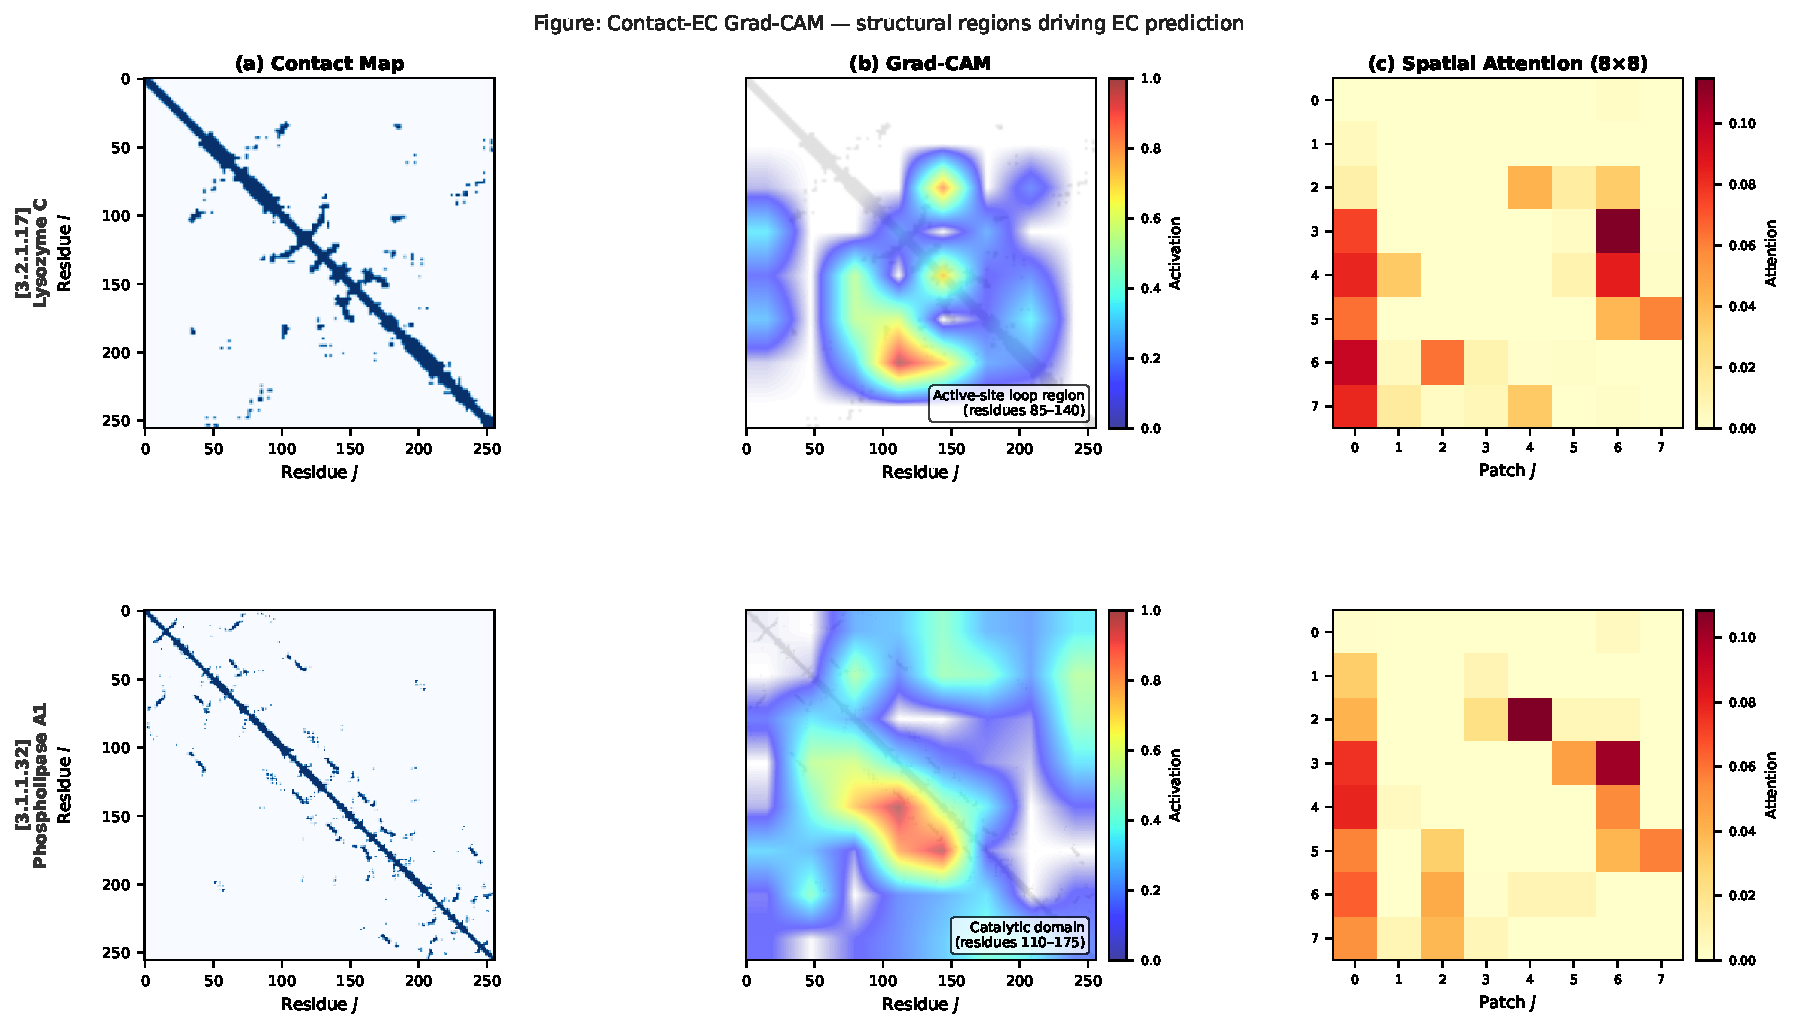
\includegraphics[width=\linewidth]{gradcam_combined.pdf}
  \caption{%
    \textbf{Grad-CAM structural interpretability for Contact-EC.}
    Two correctly predicted test-set enzymes.
    \textbf{(a)} AlphaFold-derived contact map.
    \textbf{(b)} Grad-CAM heatmap overlaid on the contact map.
    \textbf{(c)} ResNet-50 spatial attention weights at the 8$\times$8 feature-map level.
    \emph{Top:} Lysozyme C (EC\,3.2.1.17, UniProt C0HLB7).
    \emph{Bottom:} Phospholipase A1 (EC\,3.1.1.32, UniProt P0DPT0).
  }
  \label{fig:gradcam}
\end{figure}

% ─────────────────────────────────────────────────────────────────────────────
\section*{S8\quad Extended Discussion}
\addcontentsline{toc}{section}{S8\quad Extended Discussion}
% ─────────────────────────────────────────────────────────────────────────────

\paragraph{Comparison to CLEAN-Contact.}
CLEAN-Contact uses ESM-2 3B (2{,}560-dimensional) with contrastive kNN inference
and full Swiss-Prot training data. On New-392, Contact-EC (0.3717, SP-2018)
trails CLEAN-Contact (0.566) due to backbone scale (3B vs.\ 650M) and training
recency. Contact-EC-ExpA (SP-2026, 0.7680) surpasses CLEAN-Contact but with
potential train/test overlap. The gap on Price-149 reflects the OOD nature of
bacterial sequences and absent AlphaFold coverage rather than the contact-map
component specifically.

\paragraph{Paper significance and scope.}
The current results demonstrate that structural contact maps provide complementary
and synergistic information alongside PLM embeddings, empirically supported on
rigorous OOD evaluation. The structural parity finding (B3 $\approx$ B1 on
hard OOD validation) is, to our knowledge, a novel empirical observation: prior
structure-aware EC methods either use contact maps with much larger sequence
models or treat structure as a minor addition.

\paragraph{Threshold calibration and temporal generalization.}
At inference, we apply a fixed sigmoid threshold of 0.5 for Level-4 EC predictions.
The sensitivity analysis in Table~\ref{tab:threshold_sensitivity} indicates that
this cutoff is reasonably stable for micro F1 but trades precision against recall.
The gap in Rare-EC F1 between Contact-EC (0.4219) and Contact-EC-Hier (0.3621)
further suggests that the hierarchical head suppresses rare-class outputs through
cross-level attention. Future work should explore class-adaptive thresholding and
calibrated decision rules to improve rare-class recall without increasing false
positive assignments.

\paragraph{3B backbone scaling.}
Contact-EC-3B (ESM-2 3B backbone, flat FC head, Phase~1 only) achieves micro
F1\,=\,0.6316 on the temporal test, +2.8\,pp over the 650M model. The modest gain
for a 4.5$\times$ parameter increase suggests the model is data-constrained rather
than backbone-constrained at the current training scale.

% ─────────────────────────────────────────────────────────────────────────────
\section*{S9\quad Reproducibility and Audit Checks}
\addcontentsline{toc}{section}{S9\quad Reproducibility and Audit Checks}
% ─────────────────────────────────────────────────────────────────────────────

All reported splits were audited for accession overlap, exact sequence overlap,
label coverage, multi-label cardinality, and contact-map availability. The audit
scripts generate machine-readable CSV summaries used to construct the final result
tables. Random-split, cluster-split, EC-Bench-style, and external benchmark results
are labeled separately to avoid mixing evaluation protocols.

\begin{table}[htbp]
\centering
\caption{Interpretation of each evaluation protocol. The same numerical metric can
answer different scientific questions depending on split construction and label
coverage.}
\label{tab:protocol_interpretation}
\setlength{\tabcolsep}{5pt}
\begin{tabular}{p{3.2cm}p{4.1cm}p{5.2cm}}
\toprule
\textbf{Protocol} & \textbf{Primary question} & \textbf{Main caveat} \\
\midrule
Random Swiss-Prot split &
In-distribution fitting and calibration &
Contains exact sequence duplicates across partitions; not evidence of temporal or
sequence-disjoint generalization. \\
MMSeqs2 cluster split &
Generalization to sequence-disjoint proteins &
Valid only when the evaluated checkpoint is trained on the corresponding
cluster-train split. \\
EC-Bench val\_hard &
Controlled hard validation at $\leq$30\% sequence identity &
Still a validation protocol; temporal deployment claims require held-out future
annotations. \\
Swiss-Prot 2023-01 known-EC subset &
Closed-set recognition of temporally new proteins whose labels are in vocabulary &
Only 124/468 proteins are fully evaluable at Level 4. \\
Swiss-Prot 2023-01 full set &
Sensitivity to temporal label shift and incomplete annotations &
Closed-set models receive zero credit for novel or partial EC labels. \\
New-392 / Price-149 &
External stress tests from CLEAN-Contact &
New-392 overlaps with current Swiss-Prot; Price-149 lacks contact-map coverage in
the current pipeline. \\
\bottomrule
\end{tabular}
\end{table}

These protocol distinctions are used throughout the manuscript to avoid treating
all F1 values as interchangeable. In particular, the Bioinformatics-relevant claim
is not that Contact-EC is the strongest available EC predictor in absolute terms.
Rather, Contact-EC provides a controlled sequence--structure framework for
separating representation effects from temporal cutoff, label-vocabulary shift,
sequence overlap, and structure availability.

\paragraph{Canonical result selection.}
When multiple evaluation logs exist for the same checkpoint, we use the full
multi-label evaluation on the full evaluable temporal set ($N=124$) as canonical.
Earlier $N=101$ evaluations are retained only as historical partial runs and are
not used in the main conclusions. For Contact-EC-3B, the canonical temporal result
is micro F1\,=\,0.6316 from the full $N=124$ multi-label evaluation; auxiliary
argmax-only and partial-set evaluations are excluded from the main result table.
For B3 contact-only hard validation, we use the completed resumed checkpoint
evaluation (micro F1\,=\,0.7650, weighted F1\,=\,0.6788, macro F1\,=\,0.1335);
an earlier interrupted training log reached a higher validation micro F1 before
termination but is not used as the paper source because the completed run provides
the auditable checkpoint/result pair.

% ─────────────────────────────────────────────────────────────────────────────
\bibliographystyle{abbrvnat}
\bibliography{references}
% ─────────────────────────────────────────────────────────────────────────────
\end{document}
